%
% fig-zyklus.tex
%
% (c) 2025 Prof Dr Andreas Müller
%
\begin{figure}
\centering
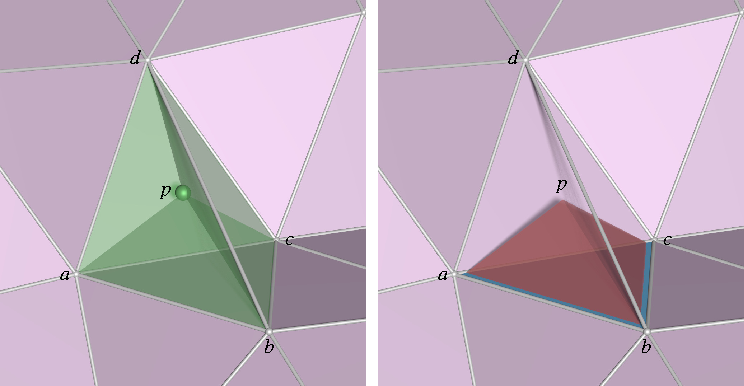
\includegraphics{chapters/120-topologie/images/zyklus.pdf}
\caption{Unterteilung des 3-Simplex $abcd$ mit dem inneren Punkt $p$
(links).
Es entstehen sechs neue 2-Simplizes ({\color{darkgreen}grün}) und vier
neue 3-Simplizes, die durch jeweils drei neue und ein ursprüngliches
2-Simplex berandet sind.
Wenn ein Zyklus (die hellrot dargestellten 2-Simplizes der ``Rückwand'')
eines der neuen 2-Simplizes enthält, dann enthält
er auch noch zwei andere, die eines der vier 3-Simplizes beranden
(rechts, rotes 3-Simplex).
Durch subtrahieren des Randes dieses 3-Simplex bleibt nur
wird der Zyklus auf einen homologen Zyklus mit dem blauen 2-Simplex
reduziert.
\label{buch:topologie:simplex:fig:zyklus}}
\end{figure}
